%% $Id: method.tex,v 1.1 2015/11/15 10:24:32 jmuelmen Exp $

%% description of the retrieval method and the evaluation using various
%% ground-based observations

%% Copernicus Publications Manuscript Preparation Template for LaTeX Submissions
%% ---------------------------------
%% This template should be used for copernicus.cls
%% The class file and some style files are bundled in the Copernicus Latex Package which can be downloaded from the different journal webpages.
%% For further assistance please contact the Copernicus Publications at: publications@copernicus.org
%% http://publications.copernicus.org


%% Please use the following documentclass and Journal Abbreviations for Discussion Papers and Final Revised Papers.


%% 2-Column Papers and Discussion Papers
\documentclass[amt,manuscript]{copernicus}\usepackage[]{graphicx}\usepackage[]{color}
%% maxwidth is the original width if it is less than linewidth
%% otherwise use linewidth (to make sure the graphics do not exceed the margin)
\makeatletter
\def\maxwidth{ %
  \ifdim\Gin@nat@width>\linewidth
    \linewidth
  \else
    \Gin@nat@width
  \fi
}
\makeatother

\definecolor{fgcolor}{rgb}{0.345, 0.345, 0.345}
\newcommand{\hlnum}[1]{\textcolor[rgb]{0.686,0.059,0.569}{#1}}%
\newcommand{\hlstr}[1]{\textcolor[rgb]{0.192,0.494,0.8}{#1}}%
\newcommand{\hlcom}[1]{\textcolor[rgb]{0.678,0.584,0.686}{\textit{#1}}}%
\newcommand{\hlopt}[1]{\textcolor[rgb]{0,0,0}{#1}}%
\newcommand{\hlstd}[1]{\textcolor[rgb]{0.345,0.345,0.345}{#1}}%
\newcommand{\hlkwa}[1]{\textcolor[rgb]{0.161,0.373,0.58}{\textbf{#1}}}%
\newcommand{\hlkwb}[1]{\textcolor[rgb]{0.69,0.353,0.396}{#1}}%
\newcommand{\hlkwc}[1]{\textcolor[rgb]{0.333,0.667,0.333}{#1}}%
\newcommand{\hlkwd}[1]{\textcolor[rgb]{0.737,0.353,0.396}{\textbf{#1}}}%
\let\hlipl\hlkwb

\usepackage{framed}
\makeatletter
\newenvironment{kframe}{%
 \def\at@end@of@kframe{}%
 \ifinner\ifhmode%
  \def\at@end@of@kframe{\end{minipage}}%
  \begin{minipage}{\columnwidth}%
 \fi\fi%
 \def\FrameCommand##1{\hskip\@totalleftmargin \hskip-\fboxsep
 \colorbox{shadecolor}{##1}\hskip-\fboxsep
     % There is no \\@totalrightmargin, so:
     \hskip-\linewidth \hskip-\@totalleftmargin \hskip\columnwidth}%
 \MakeFramed {\advance\hsize-\width
   \@totalleftmargin\z@ \linewidth\hsize
   \@setminipage}}%
 {\par\unskip\endMakeFramed%
 \at@end@of@kframe}
\makeatother

\definecolor{shadecolor}{rgb}{.97, .97, .97}
\definecolor{messagecolor}{rgb}{0, 0, 0}
\definecolor{warningcolor}{rgb}{1, 0, 1}
\definecolor{errorcolor}{rgb}{1, 0, 0}
\newenvironment{knitrout}{}{} % an empty environment to be redefined in TeX

\usepackage{alltt}



%% Journal Abbreviations (Please use the same for Discussion Papers and Final Revised Papers)

% Archives Animal Breeding (aab)
% Atmospheric Chemistry and Physics (acp)
% Advances in Geosciences (adgeo)
% Advances in Statistical Climatology, Meteorology and Oceanography (ascmo)
% Annales Geophysicae (angeo)
% ASTRA Proceedings (ap)
% Atmospheric Measurement Techniques (amt)
% Advances in Radio Science (ars)
% Advances in Science and Research (asr)
% Biogeosciences (bg)
% Climate of the Past (cp)
% Drinking Water Engineering and Science (dwes)
% Earth System Dynamics (esd)
% Earth Surface Dynamics (esurf)
% Earth System Science Data (essd)
% Fossil Record (fr)
% Geographica Helvetica (gh)
% Geoscientific Instrumentation, Methods and Data Systems (gi)
% Geoscientific Model Development (gmd)
% Geothermal Energy Science (gtes)
% Hydrology and Earth System Sciences (hess)
% History of Geo- and Space Sciences (hgss)
% Journal of Sensors and Sensor Systems (jsss)
% Mechanical Sciences (ms)
% Natural Hazards and Earth System Sciences (nhess)
% Nonlinear Processes in Geophysics (npg)
% Ocean Science (os)
% Proceedings of the International Association of Hydrological Sciences (piahs)
% Primate Biology (pb)
% Scientific Drilling (sd)
% SOIL (soil)
% Solid Earth (se)
% The Cryosphere (tc)
% Web Ecology (we)



%% \usepackage commands included in the copernicus.cls:
%\usepackage[german, english]{babel}
%\usepackage{tabularx}
%\usepackage{cancel}
%\usepackage{multirow}
%\usepackage{supertabular}
%\usepackage{algorithmic}
%\usepackage{algorithm}
%\usepackage{amsthm}
%\usepackage{float}
%\usepackage{subfig}
%\usepackage{rotating}
\usepackage{mathptmx}
%% \usepackage[T1]{fontenc}

\newcommand\comment[2]{\{\hlnum{ \textit{#1}: #2}\}}
\newcommand\commentjm[1]{\comment{$j_\mu$}{#1}}
\IfFileExists{upquote.sty}{\usepackage{upquote}}{}
\begin{document}



%% \linenumbers

\title{Using CALIOP to estimate the base height of optically thick clouds\\
%% \title{Cloud base height retrievals using 2B-GEOPROF-LIDAR and C-BREE$z$}
Used to be: ``Optimized Detection by Radar/lidAr for base of Nuages (ODR/AN)''}


% \Author[affil]{given_name}{surname}

\Author[1]{Johannes}{M\"ulmenst\"adt}
\Author[1]{Odran}{Sourdeval}
%%\Author[1]{Edward}{Gryspeerdt}
\Author[1]{Johannes}{Quaas}

\affil[1]{Institute of Meteorology, Universit\"at Leipzig, Leipzig, Germany}
\affil[2]{Anyone else?}

%% The [] brackets identify the author with the corresponding affiliation. 1, 2, 3, etc. should be inserted.



\runningtitle{Cloud base height retrievals from CALIOP}

\runningauthor{M\"ulmenst\"adt et al.}

\correspondence{Johannes M\"ulmenst\"adt (\href{mailto:johannes.muelmenstaedt@uni-leipzig.de}{johannes.muelmenstaedt@uni-leipzig.de})}



\received{}
\pubdiscuss{} %% only important for two-stage journals
\revised{}
\accepted{}
\published{}

%% These dates will be inserted by Copernicus Publications during the typesetting process.


\firstpage{1}

\maketitle



\begin{abstract}
  A measurement technique is presented that uses CALIOP lidar profiles to
  estimate cloud base heights.  The technique provides cloud base heights even
  when clouds are thick enough to attenuate the lidar beam (optical thickness
  $\tau \gtrsim 5$) by treating the cloud base height of nearby thinner clouds as
  representative of the entire cloud field.  Using ground-based ceilometer data,
  uncertainty estimates are derived as a function of various properties of the
  CALIOP lidar profiles.  Evaluation of the predicted cloud base heights and
  their predicted uncertainty using a second, statistically independent,
  ceilometer data set shows that cloud base heights and uncertainties are biased
  by less than 10\%.
\end{abstract}

\commentjm{General comments:
  \begin{itemize}
  \item switch to heights above ground $\longrightarrow$ done
  \end{itemize}
}

\introduction  %% \introduction[modified heading if necessary]
\label{sec:intro}
Cloud base height is an important geometric parameter of a cloud.  It controls
how much downwelling longwave radiation the cloud emits.  Aerosol concentration
and updraft speed at that level control the microphysics of the cloud.  It is
one of the parameters that is required in the calculation of the subadiabaticity
of the cloud.  However, due to the viewing geometry, it is also one of the most
difficult parameters to retrieve from satellite.  

Multiple methods have been proposed for satellite determination of the cloud
base height.  VIIRS cloud-base temperature method: Zhu et al.~(2014, doi
10.1002/2013GL058970).  Results of evaluating cloud base heights inferred from
oxygen absorption bands and from MISR stereoscopic images will be reported in
separate manuscripts.  For analyses wishing to combine cloud base information
with other cloud properties retrieved by A-Train satellites, these methods share
the disadvantage that the required instruments are not part of the A-Train.
Methods that are applicable to A-Train satellites are based on MODIS cloud
properties retrieved near cloud top and integrated along moist adiabats to
determine the cloud thickness (Meerk\"otter and Zinner (2007)
(10.1029/2007GL030347)) or on active remote sensing by CloudSat (2B-GEOPROF,
Marchand et al) or a combination of CloudSat and CALIOP (2B-GEOPROF-LIDAR, Mace
and Zhang 2014).  The MODIS-derived cloud thickness assumes adiabatic cloud
profiles and therefore cannot be used to constrain subadiabaticity.  CloudSat
misses the small droplets at the base of nonprecipitating clouds, and retrievals
are further degraded in the ground clutter region.  CALIOP detects the bases of
only the thinnest clouds ($\tau < 5$, according to Mace and Zhang,
10.1002/2013JD021374); frequently, it is desirable to know the base height of
thick clouds as well.

In this paper, we revisit the CALIOP cloud base determination.  Because the
lifting condensation level is approximately homogeneous within an airmass, the
cloud bases retried by CALIOP for thin clouds may be a good proxy for the cloud
base heights of an entire cloud field, including the optically thicker clouds
within the filed.  We have designed an algorithm that extrapolates the CALIOP
cloud-base measurements into locations where CALIOP attenuates before reaching
cloud base.  This algorithm is called CBASE (Cloud Base Altitude Spatial
Extrapolator).  In this paper we evaluate its performance by comparing CBASE
cloud base heights against cloud base heights observed by ground-based
ceilometers.

Section~\ref{sec:data} describes the data sources used in determining and
evaluating the cloud base height.  In Section~\ref{sec:algorithm} we describe
the algorithm and evaluate its performance, including error statistics.  We
conclude in Section~\ref{sec:conclusions} with an outlook on the longstanding
questions that this retrieval can address.

\section{Data}
\label{sec:data}

Description of the CALIOP VFM data.

The sources of ground-based observations are the following:
\begin{description}
\item[METARs] aviation routine and special weather reports (METARs) where the
  cloud base height is measured by ceilometer; to ensure that this is the case,
  we restrict ourselves to the contiguous continental United States, where the
  cloud base height is mostly derived automatically by laser ceilometers that
  form part of Automated Surface Observing Stations (ASOS)
\item[HD(CP)$^2$ ceilometers] \commentjm{Unless there is an urgent reason, these
    will have to wait for a later paper}
\item[ICOADS] \commentjm{Unless there is an urgent reason, these
    will have to wait for a later paper}
\item[R/V \textit{Polarstern} ceilometer] \commentjm{Unfortunately, there is
    only a minute number of overpasses within 100~km, mostly at high latitudes}
\item[MAGIC ceilometer] \commentjm{Unfortunately, the number of overpasses here
    is also very small; need to check that I have all the MAGIC data}
\end{description}

Description of the airport ceilometers.  METARs:
\verb+https://library.wmo.int/pmb_ged/wmo_49-v2_2013_en.pdf+; ASOS:
\verb+http://www.nws.noaa.gov/asos/pdfs/aum-toc.pdf+ 

\section{Algorithm and evaluation}
\label{sec:algorithm}

The algorithm and evaluation proceed in four steps:
\begin{enumerate}
\item We determine the cloud base height from all CALIOP profiles where the
  surface generates a return ($\longrightarrow$ lidar is not attenuated above
  cloud base).  We refer to these cloud base heights as \textit{local cloud base
    heights} in the sense that they are local to the CALIOP profile.
\item Using ground-based ceilometer data, we determine quality of cloud base
  height depending on a number of factors.  
\item Based on the predicted quality of each local cloud base, we either reject
  the local cloud base or combine it with other local cloud bases within a
  distance $D_\text{max}$ of the point of interest (POI) $\longrightarrow$
  estimate of cloud base height, estimate of cloud base height uncertainty
\item Using a statistically independent validation dataset, we verify that the
  predicted cloud base height and uncertainty are correct.
\end{enumerate}

At several points in the algorithm development, it is necessary to know the true
(ceilometer-observerd) cloud base height.  We use ceilometer observations from
the year 2008 at those points.  A statistically independent data set is required
for an unbiased evaluation of the algorithm performance; we use the year 2007.

This section is divided into four subsections, one for each algorithm step
enumerated above.

Figure~\ref{fig:method} illustrates the method.

\subsection{Determination of local cloud base height}
\label{sec:algorithm:local}
Source of local cloud base from the CALIOP VFM: any profile with a surface
return.  

\subsection{Determination of local cloud base quality}
\label{sec:algorithm:qual}
We assess the quality of the CALIOP cloud base height $z$ using the
ceilometer-observed cloud base height $\hat{z}$ using root mean square error
(RMSE), defined as
\begin{equation}
  \label{eq:rmse}
  E = \sqrt{\frac{1}{N}\sum\limits_{i = 1}^{N}\left(z_i - \hat{z}\right)^2}.
\end{equation}
The sum runs over all CALIOP profiles containing a cloud layer and a surface
return that are within 100~km horizontal distance of the ceilometer, occurred
within 3600~s of a ceilometer observation, and have their lowest CALIOP cloud
feature within 3~km of the surface.  Ceilometer observations are only used if
the observation closest in time to the Calipso overpass contains a cloud within
3~km of the surface.  A height limit is imposed because a subset of the
ceilometers has a range limit of 12500~feet, and all ceilometers report ceilings
above 10000~feet with reduced granularity (500~feet); the 3~km threshold avoids
those ceilometer limitations and mimics the ISCCP definition of low cloud
($p > 690\text{ hPa}$).

The following metrics, which are useful for a qualitative assessment of the
quality of the satellite cloud base, are also calculated, but play no
quantitative role in the algorithm:
\begin{description}
\item[Correlation coefficient] between the CALIOP cloud base and ground-based
  observation of the cloud base.  We use the Pearson correlation coefficient.
  Ideally the correlation coefficient would be unity.  
\item[Linear regression slope and intercept] (ideally 1 and 0, respectively).  
\item[Retrieval bias,] defined as
  \begin{equation}
    \label{eq:bias}
    \mbox{bias} = \frac{1}{N}\sum\limits_{i = 1}^{N}\left(z_i - \hat{z}\right),
  \end{equation}(ideally 0)
\item[Efficiency,] i.e., probability that a retrieval is available at the
  desired location (ideally 1).
\end{description}

CALIOP's ability to detect cloud base depends on the properties of the cloud.
Therefore, we expect that the cloud base height quality will vary between
different cloud profiles.  Measuring the quality as a function of various
properties of the CALIOP column may allow us to predict the quality of other
columns with the same combination of properties.  The properties that are easily
accessible in a single column and have the greatest effect on quality are:
\begin{itemize}
\item horizontal distance $D$ from the ceilometer,
\item number of column cloud bases within horizontal distance $D_\text{max}$,
\item CALIOP VFM feature quality assurance flag,
\item geometric thickness of the lowest cloud layer,
\item CALIOP thermodynamic phase determination of lowest cloud,
\item feature type, if any, detected between the lowest cloud and the surface,
\item and horizontal averaging distance required for CALIOP cloud feature
  detection.
\end{itemize}
For illustrative purposes, Figure~\ref{fig:quality-qa} shows the joint
distribution of CALIOP and ceilometer cloud base height faceted by the CALIOP
VFM feature quality assurance flag.  

Based on determining the retrieval quality one variable at a time, the following
classes of CALIOP profiles are discarded:
\begin{itemize}
\item CALIOP VFM quality assurance worse than ``high'' ,
\item ``invalid'' or ``no signal'' layers between the surface and the lowest
  cloud layer (indicating that although the surface may generate a detectable
  return, the lidar is sufficiently attenuated that the cloud base, which
  scatters less strongly than the surface, is unreliable),
\item minimum CALIOP cloud detection horizontal averaging distance within the
  lowest cloud layer greater than 1~km,
\item or phase of the lowest layer determined to be other than liquid by the
  CALIOP VFM algorithm (the reason for this is that not enough such columns
  exist to determine the RMSE reliably in each of the categories defined below).
\end{itemize}

The remaining variables are discretized roughly into quintiles with the
following boundaries:
\begin{itemize}
\item horizontal distance $D$ from the ceilometer, with boundaries 0, 40, 60,
  75, 88, and 100~km (distance greater than 100~km is discarded),
\item number of CALIOP columns $n$ with a cloud layer and a surface return
  within 100~km horizontal distance from the ceilometer, with boundaries at 0,
  175, 250, 325, 400 (multiplicities greater than 400 are accepted),
\item geometric thickness $\Delta z$ of the lowest cloud layer, with boundaries
  at 0, 0.25, 0.45, 0.625, and 1~km (thickness greater than 1~km is accepted).
\end{itemize}

We can now consider the joint distribution of CALIOP and ceilometer cloud bases
for each combination of the above variables.  (Base heights above ground are
used to remove an intrinsic correlation due to terrain.)  Because of the viewing
geometry, high CALIOP cloud bases tend to be overestimates where a higher layer
obscures a lower layer.  \commentjm{Isn't the actual reason a combination of
  regression dilution at the extremes of the distribution and phase space
  truncation at a physical boundary for low cloud bases?}  It is desirable to
correct for this bias.  The options are no correction, a linear correction
(which partially corrects for the high bias of high CALIOP base heights but
introduces a counterbias at low CALIOP base heights), and a nonlinear correction
that does not suffer from the counterbias at low CALIOP base heights.  Our
choice for nonlinear correction is a support vector machine.  The final choice
of correction is based on the performance of the three options on the tuning
sample after combination has been performed according to the next step of the
algorithm (Section~\ref{sec:algorithm:combination}).

Following bias correction, the sample RMSE is calculated for each combination of
$D$, $n$, and $\Delta z$.  The sample RMSE is taken as an estimate of the
statistical uncertainty $\sigma(D,n,\Delta z)$ on the CALIOP cloud base height.

\subsection{Combination of local cloud bases}
\label{sec:algorithm:combination}
CALIOP cloud base heights only exist sporadically \commentjm{(on average $x$\%
  of columns)}, when CALIOP happens to hit a sufficiently thin cloud.  To infer
the cloud base height $z$ at a point of interest (POI) that does not necessarily
coincide with the location of a CALIOP profile, we proceed as follows.  We first
select all local CALIOP cloud base heights within a horizontal distance
$D_\text{max} = 100$~km of the POI that satisfy the additional quality cuts
described in Section~\ref{sec:algorithm:qual}.

For each remaining local cloud base height $z_i$, we determine the predicted
uncertainty $\sigma_i$ based on the categories established in the previous
section.  We determine a combined cloud base height
\begin{equation}
  \label{eq:combo-z}
  z = \frac{\sum\limits_i^n w_i z_i}{\sum\limits_i^n w_i}
\end{equation}
with weights
\begin{equation}
  \label{eq:weights}
  w_i = \frac 1 {\sigma_i^2}
\end{equation}
(optimal weights for uncorrelated least-squares).  In practice, the individual
measurements of cloud base are highly correlated with fairly similar
$\sigma_i$.  The cloud base estimate by Eq.~(\ref{eq:combo-z}) with weights
given by Eq.~(\ref{eq:weights}) remains unbiased even in the presence of
correlations.  However, for the combined cloud base uncertainty,
the uncorrelated weights would yield a biased estimate in the presence of
correlations.  The expression
\begin{equation}
  \label{eq:combo-sigma}
  \sigma^2 = \frac 1 n \sum\limits_i^n \sigma_i^2
\end{equation}
yields acceptable results, as would be expected for highly correlated and fairly
similar $\sigma_i$.

One choice remains to be made, namely which of the bias correction methods
described in Section~\ref{sec:algorithm:qual} to apply to the local cloud base
heights before combination.  The uncorrected local base heights result in a high
bias (Figure~S1), as would be expected from the high bias on the constituent
local cloud base heights.  The linear correction, which reduces the high bias
for high cloud base heights but introduces a counterbias for low cloud base
heights, leads to a low bias in the combined base height (Figure~S2), again as
would be expected.  Among the correction methods investigated, the SVM-based
correction results in the behavior closest to the 1-to-1 line.

\subsection{Evaluation of cloud base heights and cloud base height errors}
\label{sec:algorithm:eval}




Having tuned the algorithm on data from the year 2008, we evaluate it using a
statistically independent data set from the year 2007.  In the evaluation data
set, the ``true'' (i.e., measured by the ceilometer) cloud base height $\hat{z}$
is known in addition to the estimated cloud base height $z$ and the estimated
cloud base height uncertainty $\sigma$, determined according to the procedure
described in the previous section.

For satellite-derived measurements of the cloud base height $z$ that are
unbiased with respect to the ceilometer-observed cloud base heights $\hat{z}$
and have correctly estimated uncertainties $\sigma$, the pdf of the quantity
$(z - \hat{z})/\sigma$ has zero mean and unit standard deviation. In our
evaluation data set, we find a mean of 0.03 and a standard deviation of 1.05 -- so both the cloud base estimate and
the uncertainty estimate are unbiased at the better than 10\%\ level.

Discussion of representativeness of continental clouds over North America for
the remainder of the globe.  A marine validation dataset would be very welcome. 

\section{Results and data product availability}
\label{sec:results}

Geographic distributions of mean or median cloud base and thickness.  Annual
cycle (if it's interesting).  

Comparison with 2B-GEOPROF-LIDAR cloud bases: distinguish between radar-only and
lidar-only bases (both is rare for warm cloud).  Radar-only mean error is large
because the radar cloud base height predominantly clusters around the top of the
ground clutter region with little dependence on the actual cloud base height.
Lidar-only 2B-GEOPROF-LIDAR cloud base performs about as well as the CBASE cloud
base on average, but does not provide an uncertainty estimate (and therefore no
way to select only low-uncertainty cloud base estimates).

Data is available at DKRZ or PANGEA (need to look into which one is more
appropriate).  \commentjm{Obtain DOI, put it here.}

\conclusions
\label{sec:conclusions}
\par Summary.  How useful is the cloud-base retrieval for various purposes?
There are two main cases: where accuracy is more important than efficiency, and
the other way around.  For surface radiative flux (hyperlinear in CBT), accuracy
is more important.  For geometric thickness, efficiency.  For subadiabaticity,
need to do the error propagation.

\begin{acknowledgements}
CALIOP VFM from ICARE.  Computing (and data hosting?) at DKRZ.  Funding.
\end{acknowledgements}

% \begin{table}[t]
% \caption{}
% \vskip4mm
% \centering
% \begin{tabular}{p{\parindent}l|lll|lll}
% \hline\hline
% && \multicolumn{3}{c|}{Local retrieval} & \multicolumn{3}{c}{C-BASE retrieval} \\
% && 2BGL & DARDAR & CAL & 2BGL & DARDAR & CAL \\
% \hline
% \multicolumn{2}{l|}{Efficiency} & & \\
% & METAR & \\
% & MAGIC & \\
% & \chem{HD(CP)^2} & \\
% \multicolumn{2}{l|}{Bias} & \\
% \multicolumn{2}{l|}{RMSE} \\
% \hline\hline
% \end{tabular}
% \end{table}

\begin{figure}
  \centering
  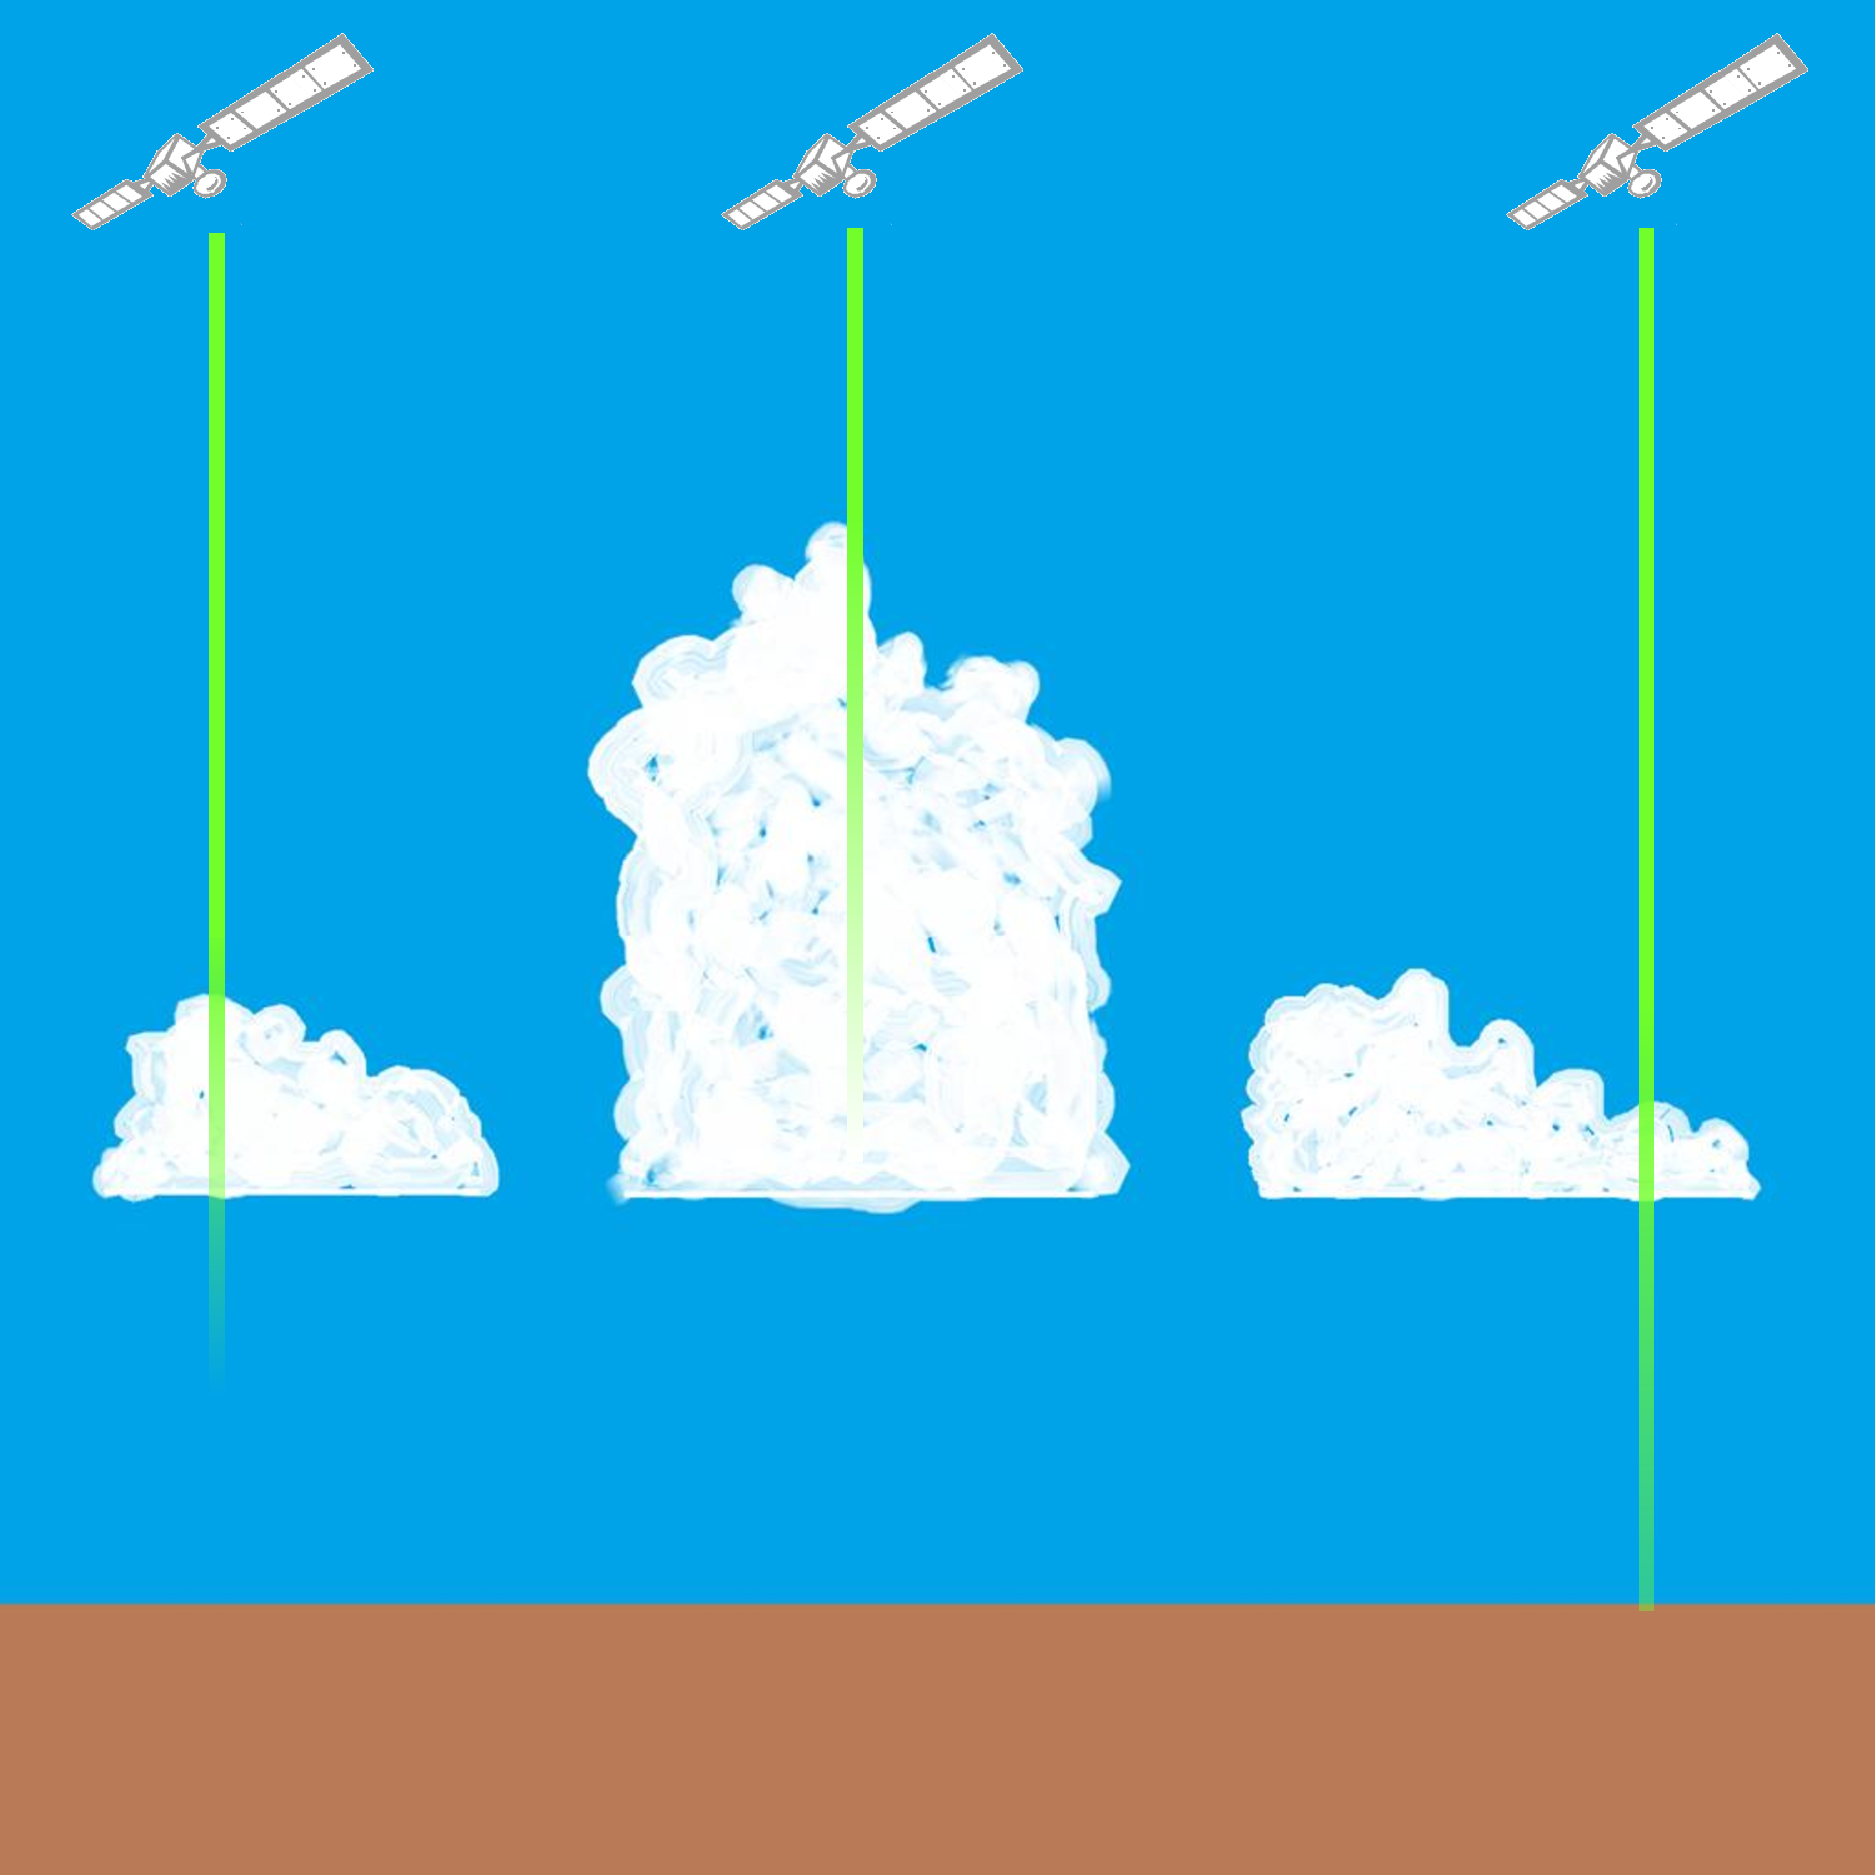
\includegraphics[width=0.5\linewidth,keepaspectratio=true]{CloudFieldCALIOP.pdf}
  \caption{Schematic of CALIOP cloud base determination and evaluation strategy.
    \commentjm{Amazing figure by Christoph.  The only way to make it even better
      would be to add a ceilometer.}}
  \label{fig:method}
\end{figure}

\begin{figure*}
  \centering
\begin{knitrout}
\definecolor{shadecolor}{rgb}{0.969, 0.969, 0.969}\color{fgcolor}

{\centering 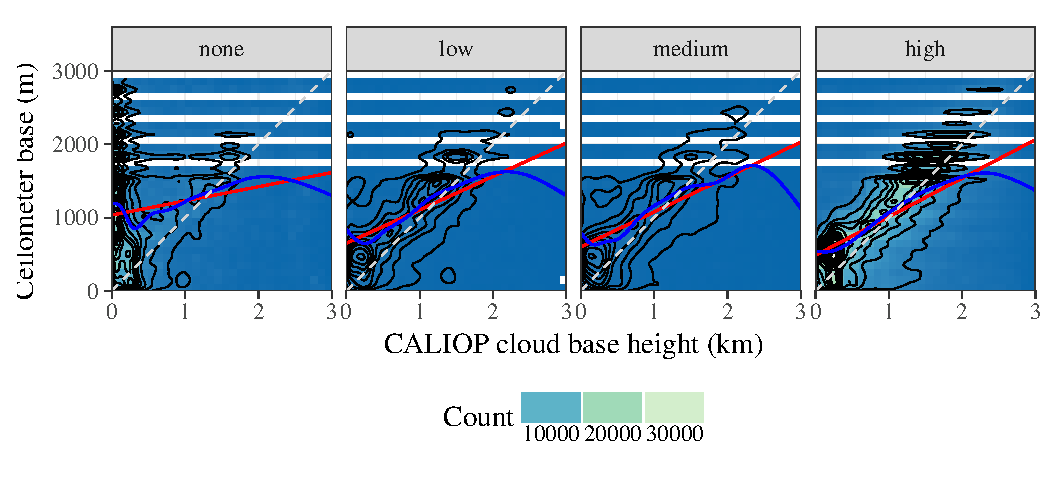
\includegraphics[width=0.95\textwidth]{figure/method-eval-qual-1} 

}



\end{knitrout}
  \caption{Scatter plots of CALIOP versus ceilometer local cloud base height
    faceted by the CALIOP VFM QA flag}
  \label{fig:quality-qa}
\end{figure*}

\begin{figure*}
  \centering
\begin{knitrout}
\definecolor{shadecolor}{rgb}{0.969, 0.969, 0.969}\color{fgcolor}

{\centering 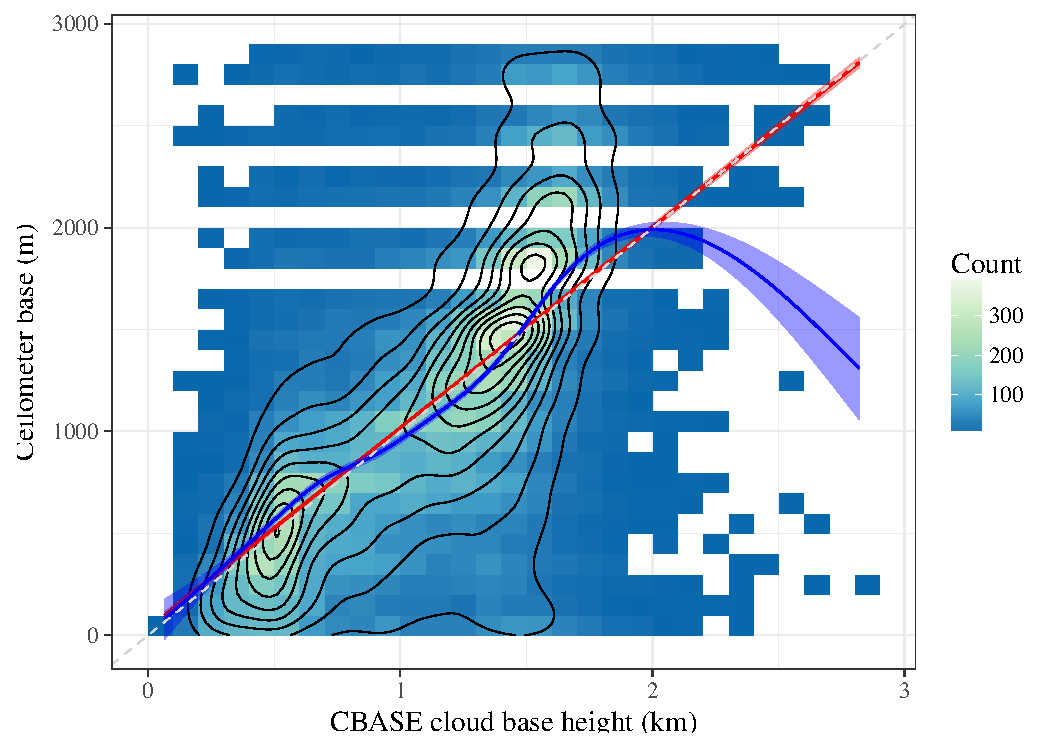
\includegraphics[width=0.95\textwidth]{figure/method-combo-plot-1} 

}



\end{knitrout}
  \caption{Scatter plot of CBASE versus ceilometer cloud base height}
  \label{fig:eval}
\end{figure*}

\begin{figure}
  \centering
\begin{knitrout}
\definecolor{shadecolor}{rgb}{0.969, 0.969, 0.969}\color{fgcolor}

{\centering 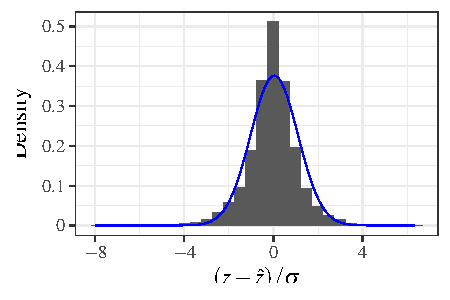
\includegraphics[width=0.5\textwidth]{figure/method-combo-eval-pull-1} 

}



\end{knitrout}
  \caption{Distribution of cloud base error divided by predicted uncertainty;
    least-squares gaussian fit with mean 0.03 and standard deviation 1.05 is overlaid.}
  \label{fig:pull}
\end{figure}

\begin{figure}
  \centering
\begin{knitrout}
\definecolor{shadecolor}{rgb}{0.969, 0.969, 0.969}\color{fgcolor}

{\centering 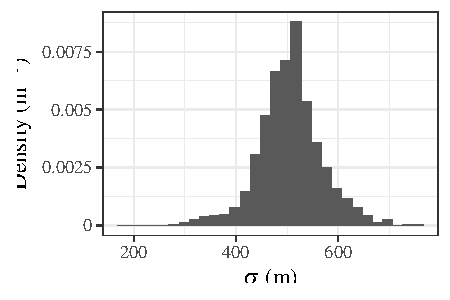
\includegraphics[width=0.5\textwidth]{figure/method-combo-eval-rmse-1} 

}



\end{knitrout}
  \caption{Distribution of predicted uncertainty}
  \label{fig:uncertainty}
\end{figure}

%% \begin{figure*}
%%   \centering
%%   <<combo-plot-rmseclass,dev='tikz',fig.width=7,fig.height=5,out.width='0.95\\textwidth',message=FALSE,cache=FALSE,results='hide',echo=FALSE>>=
%%   @
%%   \caption{Scatter plot of CBASE versus ceilometer cloud base height for
%%     different classes of predicted uncertainty}
%%   \label{fig:rmseclass}
%% \end{figure*}

\begin{table*}[t]
  \centering
  \caption{CBASE cloud base statistics by decile of predicted uncertainty}
  \label{tab:rmseclass}

% latex table generated in R 3.2.3 by xtable 1.8-3 package
% Mon May  8 15:03:11 2017
\begin{tabular}{lrrrrl}
  \hline
\hline
pred.rmse & $n$ & $r$ & RMSE (m) & bias (m) & fit \\ 
  \hline
(187,436] & 2624 & 0.749 & 403. & $-$33.2 & $y = 1.14 x - 63.5$ m \\ 
  (436,461] & 2624 & 0.722 & 429. & $-$26.4 & $y = 1.20 x - 186.$ m \\ 
  (461,478] & 2624 & 0.725 & 460. & $-$26.3 & $y = 1.25 x - 256.$ m \\ 
  (478,492] & 2624 & 0.693 & 466. & $-$29.4 & $y = 1.19 x - 182.$ m \\ 
  (492,506] & 2635 & 0.616 & 512. & $-$0.0279 & $y = 1.14 x - 157.$ m \\ 
  (506,517] & 2721 & 0.564 & 550. & $-$12.7 & $y = 1.14 x - 157.$ m \\ 
  (517,530] & 2516 & 0.566 & 562. & $-$0.809 & $y = 1.11 x - 131.$ m \\ 
  (530,550] & 2624 & 0.566 & 569. & $-$29.9 & $y = 1.15 x - 150.$ m \\ 
  (550,582] & 2624 & 0.497 & 640. & $-$11.8 & $y = 1.06 x - 66.1$ m \\ 
  (582,764] & 2624 & 0.446 & 716. & 13.1 & $y = 0.977 x + 14.6$ m \\ 
   \hline
\hline
\end{tabular}

\end{table*}

\begin{figure*}
  \centering

\begin{knitrout}
\definecolor{shadecolor}{rgb}{0.969, 0.969, 0.969}\color{fgcolor}

{\centering 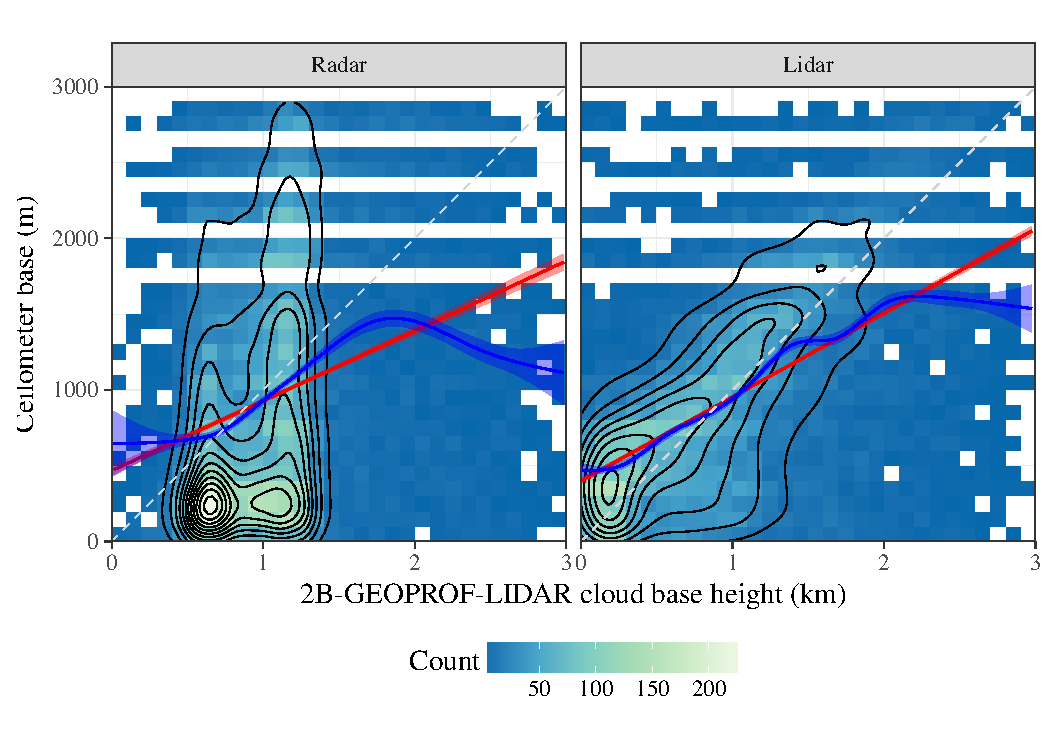
\includegraphics[width=0.95\textwidth]{figure/method-eval-2bgeoprof-1} 

}



\end{knitrout}
  %%<<eval-2bgeoprof-tbl,dev='tikz',fig.width=9.1,fig.height=4.5,out.width='\\textwidth',message=FALSE,cache=TRUE,echo=FALSE,results='asis'>>=
  %%@
  \caption{Scatter plot of 2B-GEOPROF-LIDAR versus ceilometer cloud base
    height.  \commentjm{I \textit{think} this uses Claudia's algorithm (minimum
      cloud base within $D_\text{max}$), but I have to check.}}
  \label{fig:eval-2b}
\end{figure*}

\begin{figure*}
  \centering
  %% <<vis-cbase,cache=TRUE,echo=FALSE,results='hide'>>=
  %% @
  %% <<vis-cbase2,dev='tikz',fig.width=7,fig.height=5,out.width='0.95\\textwidth',message=FALSE,cache=TRUE,echo=FALSE,results='hide'>>=
  %% @
  \caption{Geographic distribution of median cloud bases and median cloud
    thicknesses \commentjm{Make the figure less complex.  One panel with overall
    CBH.}}
  \label{fig:geo}
\end{figure*}




\end{document}
